% formal/stateless.tex
% mainfile: ../perfbook.tex
% SPDX-License-Identifier: CC-BY-SA-3.0

\section{Stateless Model Checkers}
\label{sec:formal:Stateless Model Checkers}
%
\epigraph{He's making a list, he's permuting it twice\dots}
	{\emph{with apologies to Haven Gillespie and J. Fred Coots}}

앞 섹션에서 설명한 SAT 풀이기 접근법은 상당히 편리하고 강력하지만, 상태를
포함한 모든 가능한 수행을 완전히 따라가는 것은 상당한 오버헤드를 일으킵니다.
실제로, 이 메모리와 CPU 시간 오버헤드는 적당하게 검증될 수 있는 프로그램의
크기를 급격하게 제한할 수 있는데, 이는 더 큰 프로그램에서는 덜 정확한 접근법이
버그를 찾을 수도 있을까 하는 질문을 일으킵니다.

\iffalse

The SAT-solver approaches described in the previous section are quite
convenient and powerful, but the full tracking of all possible
executions, including state, can incur substantial overhead.
In fact, the memory and CPU-time overheads can sharply limit the size
of programs that can be feasibly verified, which raises the question
of whether less-exact approaches might find bugs in larger programs.

\fi

\begin{figure}[tbp]
\centering
\resizebox{2.1in}{!}{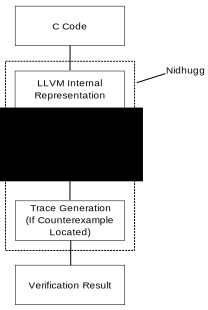
\includegraphics{formal/nidhugg}}
\caption{Nidhugg Processing Flow}
\label{fig:formal:Nidhugg Processing Flow}
\end{figure}

여전히 배심원들은 이 질문에 대해 고민 중이지만,
Nidhugg~\cite{CarlLeonardsson2014Nidhugg} 와 같은 stateless 모델 검사기들은
Figure~\ref{fig:formal:Nidhugg Processing Flow} 에 보인 것처럼 몇몇 경우에
비슷한 수준의 쉬운 사용성을 가지고 더 큰 프로그램들을
처리했습니다~\cite{SMC-TreeRCU}.
또한, Nidhugg 는 리눅스 커널 RCU 검증 시나리오에서 \co{cbmc} 보다 수십배
빨랐습니다.
물론, Nidhugg 의 속도와 확장성 이득은 그게 데이터 비결정성을 처리하지 않는다는
사실에서 나옵니다만, 이 특정 검증 시나리오에서는 중요한 게 아니었습니다.

그렇다고 하나, \co{cbmc} 에서와 같이 Nidhugg 는 리눅스 커널 RCU 메인테이너가
아직 몰랐던 버그를 찾지는 못했습니다.
그러나, 리눅스 커널 RCU 의 한 역사적 버그는 그 메인테이너의 생각과 다른 커밋에
의해 수정되었음을 보이는 게 가능했는데, 이는 Nidhugg 와 같은 stateless 모델
검사기가 언젠가는 병렬 코드의 동시성 버그를 찾는데 유용해질 것이라는 추가적
희망을 갖게 해줍니다.

\iffalse

Although the jury is still out on this question, stateless model
checkers such as Nidhugg~\cite{CarlLeonardsson2014Nidhugg} have in
some cases handled larger programs~\cite{SMC-TreeRCU}, and with
similar ease of use, as illustrated by
Figure~\ref{fig:formal:Nidhugg Processing Flow}.
In addition, Nidhugg was more than an order of magnitude faster than
was \co{cbmc} for some Linux-kernel RCU verification scenarios.
Of course, Nidhugg's speed and scalability advantages are tied to
the fact that it does not handle data non-determinism, but this
was not a factor in these particular verification scenarios.

Nevertheless, as with \co{cbmc}, Nidhugg has not yet been able to
locate a bug that Linux-kernel RCU's maintainer was not already
aware of.
However, it was able to demonstrate that one historical bug in
Linux-kernel RCU was fixed by a different commit than the maintainer
thought, which gives some additional hope that stateless model checkers
like Nidhugg might someday be useful for finding concurrency bugs in
parallel code.

\fi
